\subsection{Action of the Hamiltonian}

As we have now defined what we mean by the Hamiltonian \eqref{VecZ2Hamiltonian}
\begin{equation*}
H=-\sum \frac{1}{\sqrt{2}}
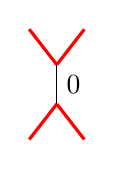
\begin{tikzpicture}[scale=0.5,baseline=(current bounding box.center)]
\draw[red,line width=0.4mm] (0,0) -- (-0.7,0.9);
\draw[red,line width=0.4mm] (0,0) -- (0.7,0.9);
\draw (0,0) to node[right] {$0$} (0,-1);
\draw[red,line width=0.4mm] (0,-1) -- (-0.7,-1.9);
\draw[red,line width=0.4mm] (0,-1) -- (0.7,-1.9);
%			\node at (0.8,1.1) {$*$};
%			\node at (-0.8,1.1) {$*$};
%			\node at (0.8,-2.1) {$*$};
%			\node at (-0.8,-2.1) {$*$};
\end{tikzpicture}
\end{equation*}
\noindent
we can study its action on the chain. For this purpose, we first need to change the basis using the identity
	\begin{equation}
		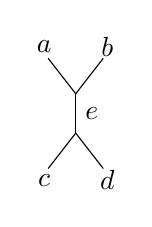
\begin{tikzpicture}[scale=0.5,baseline=(current bounding box.center)]
			\draw (0,0) -- (-0.7,0.9);
			\draw (0,0) -- (0.7,0.9);
			\draw (0,0) to node[right] {$e$} (0,-1);
			\draw (0,-1) -- (-0.7,-1.9);
			\draw (0,-1) -- (0.7,-1.9);
			\node at (0.8,1.2) {$b$};
			\node at (-0.8,1.2) {$a$};
			\node at (0.8,-2.2) {$d$};
			\node at (-0.8,-2.2) {$c$};
		\end{tikzpicture}=\sum_f\left(F_d^{abc}\right)_{ef}
		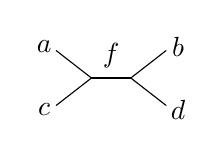
\begin{tikzpicture}[scale=0.5,baseline=(current bounding box.center)]
			\draw (0,0) -- (-0.9,0.7);
			\draw (0,0) -- (-0.9,-0.7);
			\draw (0,0) to node[above] {$f$} (1,0);
			\draw (1,0) -- (1.9,0.7);
			\draw (1,0) -- (1.9,-0.7);
			\node at (-1.2,0.8) {$a$};
			\node at (-1.2,-0.8) {$c$};
			\node at (2.2,0.8) {$b$};
			\node at (2.2,-0.8) {$d$};
		\end{tikzpicture}
	\end{equation}
which yields
	\begin{align}
		H&=-\sum \frac{1}{\sqrt{2}}\left(\left(F_*^{***}\right)_{00}
		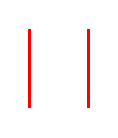
\begin{tikzpicture}[scale=0.5,baseline=(current bounding box.center)]
			\draw[red,line width=0.4mm] (0,0) -- (0,2);
			\draw[red,line width=0.4mm] (1.5,0) -- (1.5,2);
		\end{tikzpicture}+\left(F_*^{***}\right)_{01}
		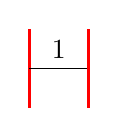
\begin{tikzpicture}[scale=0.5,baseline=(current bounding box.center)]
			\draw[red,line width=0.4mm] (0,0) -- (0,2);
			\draw (0,1) to node[above] {$1$} (1.5,1);
			\draw[red,line width=0.4mm] (1.5,0) -- (1.5,2);
		\end{tikzpicture}\ \right)\\
		&=-\sum\frac{1}{\sqrt{2}}\left(\ 
		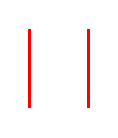
\begin{tikzpicture}[scale=0.5,baseline=(current bounding box.center)]
			\draw[red,line width=0.4mm] (0,0) -- (0,2);
			\draw[red,line width=0.4mm] (1.5,0) -- (1.5,2);
		\end{tikzpicture}+
		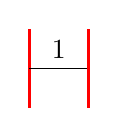
\begin{tikzpicture}[scale=0.5,baseline=(current bounding box.center)]
			\draw[red,line width=0.4mm] (0,0) -- (0,2);
			\draw (0,1) to node[above] {$1$} (1.5,1);
			\draw[red,line width=0.4mm] (1.5,0) -- (1.5,2);
		\end{tikzpicture}\ \right),
	\end{align}
where we have used the $F$ symbols we have computed above. Now we study how this Hamiltonian acts on the valid local configurations
	\begin{figure}[H]
		\begin{tikzpicture}[scale=1,baseline=(current bounding box.center)]
			\draw (-0.5,0) -- (0,0);
			\draw [red, line width=0.25mm] (0,0) -- (1,0);
			\draw (1,0) -- (1.5,0);
			\draw [red, line width=0.25mm] (0,0) -- (0,1);
			\draw [red, line width=0.25mm] (1,0) -- (1,1);
			\node at (-0.7,0) {$a$};
			\node at (1.7,0) {$b$};
		\end{tikzpicture} \hspace{20pt}
		\begin{tikzpicture}[scale=1,baseline=(current bounding box.center)]
			\draw [red, line width=0.25mm] (-0.5,0) -- (0,0);
			\draw (0,0) -- (1,0);
			\draw [red, line width=0.25mm] (1,0) -- (1.5,0);
			\draw [red, line width=0.25mm] (0,0) -- (0,1);
			\draw [red, line width=0.25mm] (1,0) -- (1,1);
			\node at (-0.7,0) {$a$};
			\node at (1.7,0) {$b$};
		\end{tikzpicture}
	\end{figure}
\noindent
The first term of the Hamiltonian leaves the configurations invariant, while the second term acts in the following way:
	\begin{align}
		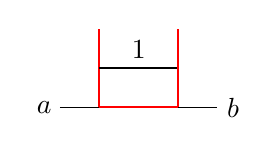
\begin{tikzpicture}[scale=1,baseline=(current bounding box.center)]
			\draw (-0.5,0) -- (0,0);
			\draw [red, line width=0.25mm] (0,0) -- (1,0);
			\draw (1,0) -- (1.5,0);
			\draw [red, line width=0.25mm] (0,0) -- (0,1);
			\draw (0,0.5) to node[above] {$1$} (1,0.5);
			\draw [red, line width=0.25mm] (1,0) -- (1,1);
			\node at (-0.7,0) {$a$};
			\node at (1.7,0) {$b$};
		\end{tikzpicture}&=
		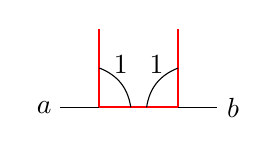
\begin{tikzpicture}[scale=1,baseline=(current bounding box.center)]
			\draw (-0.5,0) -- (0,0);
			\draw [red, line width=0.25mm] (0,0) -- (1,0);
			\draw (1,0) -- (1.5,0);
			\draw [red, line width=0.25mm] (0,0) -- (0,1);
			\draw [red, line width=0.25mm] (1,0) -- (1,1);
			\node at (-0.7,0) {$a$};
			\node at (1.7,0) {$b$};
			\draw (0,0.5) to[bend left] node[above] {$1$} (0.4,0);
			\draw (1,0.5) to[bend right] node[above] {$1$} (0.6,0);
		\end{tikzpicture}=(-1)^{a+b}
		\begin{tikzpicture}[scale=1,baseline=(current bounding box.center)]
			\draw (-0.5,0) -- (0,0);
			\draw [red, line width=0.25mm] (0,0) -- (1,0);
			\draw (1,0) -- (1.5,0);
			\draw [red, line width=0.25mm] (0,0) -- (0,1);
			\draw [red, line width=0.25mm] (1,0) -- (1,1);
			\node at (-0.7,0) {$a$};
			\node at (1.7,0) {$b$};
		\end{tikzpicture}\equiv Z_a\otimes Z_b\\
		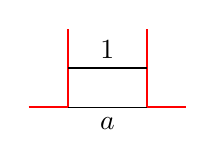
\begin{tikzpicture}[scale=1,baseline=(current bounding box.center)]
			\draw [red, line width=0.25mm] (-0.5,0) -- (0,0);
			\draw (0,0) to node[below] {$a$} (1,0);
			\draw [red, line width=0.25mm] (1,0) -- (1.5,0);
			\draw [red, line width=0.25mm] (0,0) -- (0,1);
			\draw [red, line width=0.25mm] (1,0) -- (1,1);
			\draw (0,0.5) to node[above] {$1$} (1,0.5);
		\end{tikzpicture}&=
		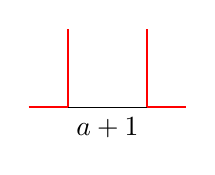
\begin{tikzpicture}[scale=1,baseline=(current bounding box.center)]
			\draw [red, line width=0.25mm] (-0.5,0) -- (0,0);
			\draw (0,0) to node[below] {$a+1$} (1,0);
			\draw [red, line width=0.25mm] (1,0) -- (1.5,0);
			\draw [red, line width=0.25mm] (0,0) -- (0,1);
			\draw [red, line width=0.25mm] (1,0) -- (1,1);
		\end{tikzpicture}\equiv X_a
	\end{align}
Hence, in general the local Hamiltonian $h_i$ acts like
	\begin{align*}
		h_i \left(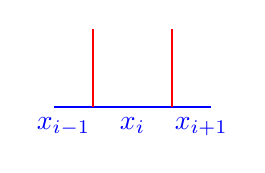
\begin{tikzpicture}[scale=1,baseline=(current bounding box.center)]
		\draw [blue, line width=0.25mm] (-0.5,0) to node[below, near start] {$x_{i-1}$} (0,0);
		\draw [blue, line width=0.25mm] (0,0) to node[below] {$x_i$} (1,0);
		\draw [blue, line width=0.25mm] (1,0) to node[below, near end] {$x_{i+1}$} (1.5,0);
		\draw [red, line width=0.25mm] (0,0) -- (0,1);
		\draw [red, line width=0.25mm] (1,0) -- (1,1);
		\end{tikzpicture}\right)=&\left(\left(Z_{x_{i-1}}\oplus 0\right)\otimes\left(0\oplus\lvert*\rangle_{x_i}\langle*\rvert\right)\otimes\left(Z_{x_{i+1}}\oplus 0\right)\right.\\&+\left.\left(0\oplus\lvert*\rangle_{x_{i-1}}\langle*\rvert\right)\otimes\left(Z_{x_i}\oplus 0\right)\otimes\left(0\oplus \lvert *\rangle_{x_{i-1}}\langle *\rvert\right)\right)\left(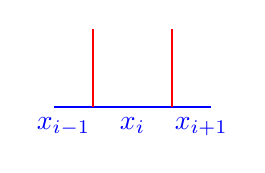
\begin{tikzpicture}[scale=1,baseline=(current bounding box.center)]
		\draw [blue, line width=0.25mm] (-0.5,0) to node[below, near start] {$x_{i-1}$} (0,0);
		\draw [blue, line width=0.25mm] (0,0) to node[below] {$x_i$} (1,0);
		\draw [blue, line width=0.25mm] (1,0) to node[below, near end] {$x_{i+1}$} (1.5,0);
		\draw [red, line width=0.25mm] (0,0) -- (0,1);
		\draw [red, line width=0.25mm] (1,0) -- (1,1);
		\end{tikzpicture}\right).
	\end{align*}
Fixing boundary conditions to $*$ freezes out half of the valid configurations, which results in the Ising model.